\chapter{Methods for inferring pairwise co-location}

With the data extracted and formatted in suitable manner, as described in the previous chapter, we move on to the main part of the thesis. Given a set of consecutive Bluetooth RSSI measurements, \textit{can we infer co-location?}; and if yes, what is the best way of doing it? 

One way of answering these questions is to simply set a threshold, and split the dataset into two parts: the ones that are above the threshold indicate co-location, while the other do not. That is exactly what \textit{Sekara,Lehmann} did in \cite{vedran}, with convincing results. They set the threshold to \textit{ -80 dBm}. 

On a similar note, we average our two types of data, the ones tagged \textit{yes} and \textit{no}, and we obtain an average of \textit{-64 dBm} for the ones tagged \textit{yes} and an average of {-82 dBm} for the ones tagged \textit{no}. From this result, one can easily see the similarity between the threshold in \textit{Sekara,Lehmann}'s work and the values obtained through this thesis's data, further indicating the validity of this result. 

The above method can successfully be used under any type of measurements. However, it does not take advantage of the additional information that our method of data gathering has provided, such as temporal information, or the significance of continuous measurements. Below we propose three methods of inferring pairwise co-location in the form of three machine learning algorithms. For each one we will provide a theoretical overview and implementation details. The chapter will end with a comparison between the three algorithms where results, ease of use and performance will be taken into consideration. 

While the parameters and the inputs used differ from one algorithm to another, one thing that remains constant across all of them is the testing methodology, described in the following section.

\section{Testing methodology}

In order to test the accuracy of the algorithms, we use cross-validation, a well recognized method for computing accuracy estimations \cite{kohavi1995study}. The technique is used here for obtaining an accuracy score for each algorithm and its variations, so that a comparison can be made at the end. Broadly speaking, cross-validation refers to the techniques used to partition the main dataset into two sets: a \textit{training} set, used in the initial phase for training the algorithms, and a \textit{testing} set, used for validating the algorithm with \textit{unseen before} data, after the training has finished. Two methods were used: k-fold validation, with $k = 10$ \cite{kohavi1995study}, and repeated random sub-sampling validation, with a $80-20$ proportion \cite{segaran}. 

\begin{itemize}
  \item K-fold validation is done by partitioning the data in k sets. One set is used for testing, while the the other $k-1$ are used for training. The processed is repeated $k$ times, once for each partition. The end result is the average over all $k$ results obtained. 
  \item For random sub-sampling validation, the dataset is partitioned into two sets. The entries are randomly assigned to one of the sets based on the proportion established at the beginning. For this type of validation, the test has been repeated 100 times, and the results averaged.   
\end{itemize}

During the execution of the tests, both k-fold validation and repeated random sub-sampling validation output extremely similar results, most of the time the results having a less than $0.5\%$ difference between them. For this reason, when presenting an algorithm score, that score will be the average of the two methods. 


\section{Neural Networks}

A first approach aims to use artificial neural networks (ANN) in order to infer co-location. Specifically, this section will deal with feed-forward ANNs, both from a theoretical and a practical point of view. 

\subsection{Theoretical overview}

The introduction of backpropagation by Rumelhart et al. \cite{rumelhart} paved the way for the development of the modern artificial neural network. In their current form, ANNs can be described as a set of processing units, called \textit{neurons}, or \textit{artificial neurons} that communicate between each other. 

The general layout of a feed-forward ANN can be seen in Fig. \ref{pic:ann}. It consists of an input layer, one or more hidden layers and an output layer. The number of \textit{neurons} on the input layer is equal with the number of features that represent the object we need to classify. The number of \textit{neurons} in the output layer usually equals the number of classes the objects need to be classified in. The number of hidden layers, and the number of \textit{neurons} in those layers varies greatly from problem to problem, and will be discussed in the next section, which tackles the implementation details.
In addition to the processing units, the other major components of a feed-forward network are the links between the \textit{neurons}. They type of ANN described here is feed-forward, which means the links are uni-directional. Information only moves from the input \textit{neurons}, to the \textit{neurons} in the hidden layers, to the \textit{neurons} in the output layers. For example, in Fig. \ref{pic:ann}, information only moves from left to right \cite{annintroduction2}.  

\begin{figure}[h]
	\begin{center}
		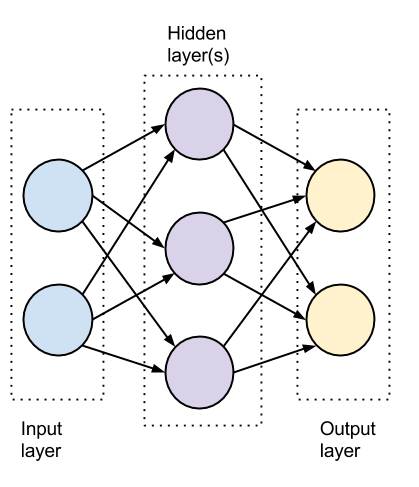
\includegraphics[scale=0.6]{figures/ANN.png}
	\end{center}
	
	\caption{General structure of an ANN.}
	\label{pic:ann}

\end{figure} 

An artificial neural network gets its name from the similarity it has with the biological network of neurons one finds in the human or animal brain. The same can be said about the way it works. Each \textit{artificial neuron} receives an input from all the other \textit{neurons} on the previous layer (or they receive outside input if they are on the input layer). Once all the inputs are received, the \textit{neuron} in question processes them and outputs the result to \textit{neurons} on the next layer \cite{annintroduction}. Fig. \ref{pic:neuron} shows the details of an \textit{artificial neuron}.

\begin{figure}[h]
	\begin{center}
		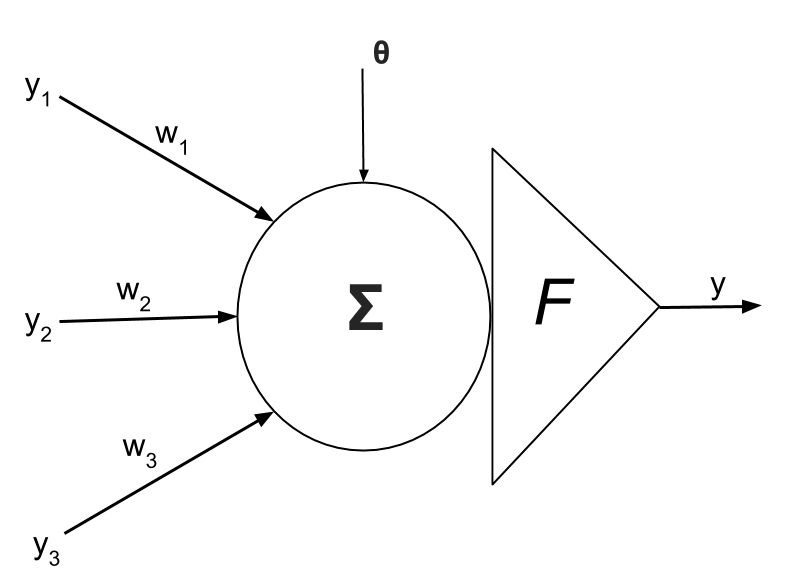
\includegraphics[scale=0.3]{figures/neuron.png}
	\end{center}
	
	\caption{Structure of an artificial neuron.}
	\label{pic:neuron}

\end{figure}

Each link between \textit{neurons} is characterized by a weight, $w_i$. A \textit{neuron} applies a so-called \textit{activation function} on the weighted sum of the inputs, and outputs the result. Sometimes, a bias is used: $\theta$. Thus, the output of single \textit{neuron} can be expressed as:

\begin{equation*}
y = F(\sum_i w_i y_i + \theta)
\end{equation*}

\begin{description}
  \item[$y$]   The output of the current \textit{neuron}.
  \item[$F$]   The activation function. This is usually either the \textit{sigmoid} function, $y = F(x) = \frac{1}{1 + e^{-x}}$, or the \textit{tanh} function \cite{annintroduction}.
  \item[$w_i$] The weight of an input link.
  \item[$y_i$] The input, either from a previous layer of \textit{neurons}, or a from outside the network.
  \item[$\theta$] Bias
\end{description}

In order for the network to output the expected result when presented with an input, it has to be set up. That translates into assigning appropriate values to the weights corresponding to the links between \textit{neurons}. One way of doing this is to manually assign the values. However, this implies a priori knowledge, which is not possible in most cases. The other choice is to \textit{train} the network. 

The training method used here is backpropagation, first introduced in \cite{rumelhart}. The intuition behind is as follows. We randomly assign values to the weights $w_i$ in the ANN. We apply an input to the network, whose result we already know, and compare the outputted result with the correct one. The aim is to minimize the difference. 

While the mathematical procedure through which researchers have reached backpropagation is outside the scope of this thesis, based on \cite{annintroduction} we will present the general equations used in the implementation of the algorithm:

We modify each weight with:  
\begin{equation*}
\Delta w_k = \alpha \delta_k y_k
\end{equation*}

Where $\alpha$ is the learning rate, $y_k$ is the input value on link $k$, and $\delta_k$ is computed as follows:
\begin{equation*}
\delta_k = F'( \sum_i w_i y_i + \theta ) \sum \delta_l w_{kl}
\end{equation*}

Where $\delta_l$ is used in the next layer, and $w_{kl}$ represents a weight between the current layer and the next one. This process continues recursively, until we reach the output layer. In order to finish the computations, we need the $\delta_o$ which corresponds to the output layer:  

\begin{equation*}
\delta_o = (d - y) F'(\sum_i w_i y_i + \theta)
\end{equation*}

Where $d$ represents the expected output, and $y$ the desired output. As one can easily see, we begin from the output layer with computing $\delta_o$, and updating the corresponding weights. We then move further one layer, and compute the corresponding $\delta$ values. We continue to go back until we reach the links that connect to the input layer. From this procedure the \textit{back} in \textit{backpropagation} comes from. 

\subsection{Implementation}

For implementation purposes we used a Python neural network, available at \cite{issam}. The network used has, besides the mandatory input and output layers a single hidden layer (which is enough \cite{Hornik1989359,Hartman,cybenko}). 

The number of \textit{neurons} in the hidden layer differs greatly from problem to problem, with some authors suggesting any number between the number of neurons in the input layer, to two times that value \cite{Stathakis}. Due to the relatively small number of features extracted from the phone data, we have run tests varying numbers of hidden units. 

During the testing, different values for the $\alpha$ parameter have been tried, in the end, the value that yielded the best results being 0.2. As such, all the tests that are done below are done with an $\alpha$ parameter of 0.2.

We begin our testing with the most basic case. We use a single feature, the measured Bluetooth RSSI. The plot in Fig.~\ref{pic:ann_single} details the results obtained. While the accuracy is acceptable, we can easily see that varying the number of hidden nodes in the hidden layer has no impact on the result. 

\begin{figure}[h]
	\begin{center}
		\includegraphics[scale=0.3]{figures/ann_single.png}
	\end{center}
	
	\caption{Test accuracy for ANN when just the RSSI is used as a feature.}
	\label{pic:ann_single}

\end{figure}

Next we try to make use of the notion of chains, as it was defined in Section~\ref{sec:data_merger}. When trying to infer co-location for a specific time window, we also look at the RSSI of the windows that are in the same chain, but before it. We gradually increased the number of \textit{neurons} in the hidden layer, as well as the number of windows we take into consideration. As we increased the number of windows, the length of the chains became a problem. Different chains have different lengths, but the number of features in the ANN remains constant. For example, when using four previous windows, and a chain has only a length of three, even in the best case scenario, we still have two missing features. 

One way to deal with this problem is to simply discard the cases that are missing values. However, this introduces significant bias into the data, as observation of the dataset has shown that shorter chains are more likely to belong to the category tagged with \textit{no}. By discarding them, we greatly reduce the number of samples tagget with \textit{no}, thus unbalancing the overall proportion of training and testing data. As such, we used imputation to replace the missing values. Two approaches were used.

A first approach used mean imputation. We replaced the missing data with the average of the values in the chain. Fig.~\ref{pic:ann_params1} shows the results obtained. Secondly, we used last observation carry forward \cite{locf}, as it involved ordered by time values. The results can be seen in Fig.~\ref{pic:ann_params2}. Consideration has been given to multiple imputation \cite{rubin2009multiple}, however, its cost, and the next result made it unsuitable.  

\begin{figure}[h]
	\begin{center}
		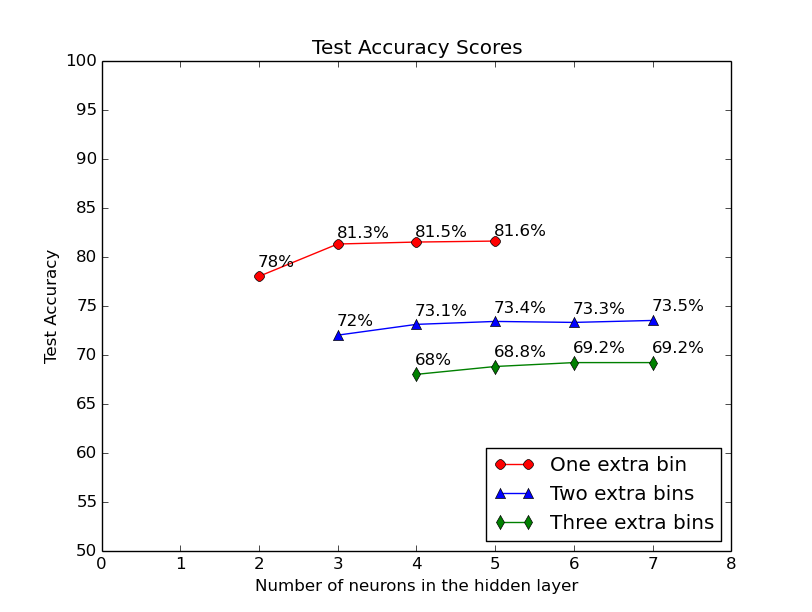
\includegraphics[scale=0.3]{figures/ann_params1.png}
	\end{center}
	
	\caption{Test accuracy for ANN when the RSSI for the current and previous time windows are used as features, with mean imputation.}
	\label{pic:ann_params1}

\end{figure}

\begin{figure}[h]
	\begin{center}
		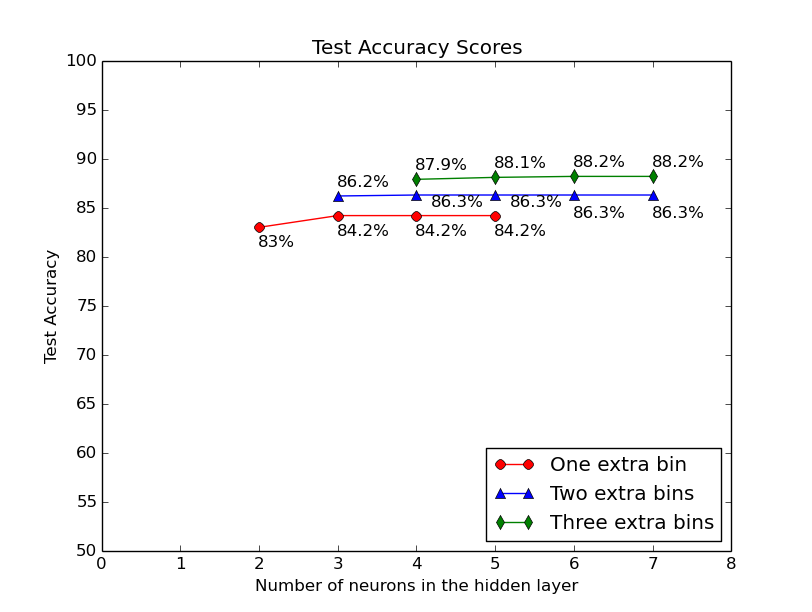
\includegraphics[scale=0.3]{figures/ann_params2.png}
	\end{center}
	
	\caption{Test accuracy for ANN when the RSSI for the current and previous time windows are used as features, with last observation carry forward imputation.}
	\label{pic:ann_params2}

\end{figure}

Taking into account the additional information provided by the chain that a window belongs to clearly improves the result. However, the previous approach had a number of issues. For the next set of parameters, we only use two features: the RSSI of the current window, and the length of the chain the window is a part of. This has the strength of avoiding any bias introduced by imputation, while at the same time making almost full use of the additional information provided by the chain. Fig.~\ref{pic:ann_chain} shows the test accuracy for this choice of features.

\begin{figure}[h]
	\begin{center}
		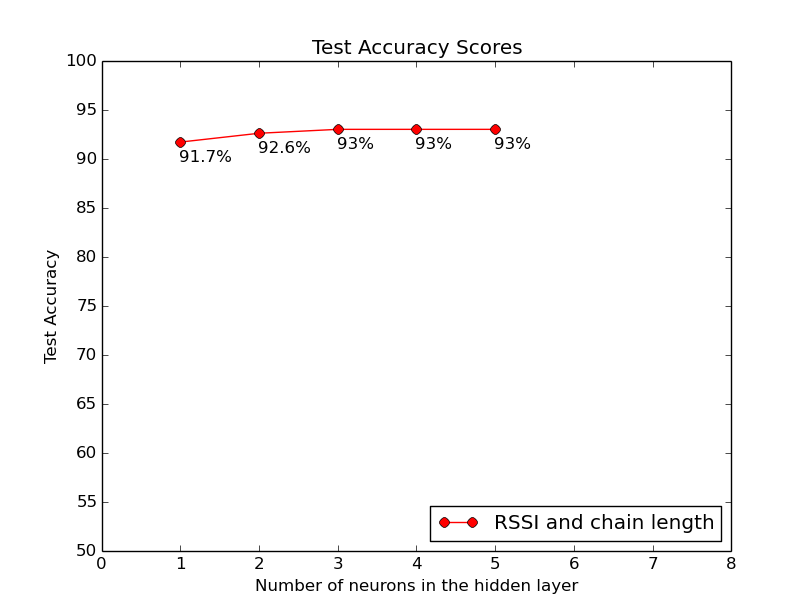
\includegraphics[scale=0.3]{figures/ann_chain.png}
	\end{center}
	
	\caption{Test accuracy for ANN when the RSSI and the chain length are used as features.}
	\label{pic:ann_chain}

\end{figure}     

\section{Regressive data}

\subsection{Theoretical overview}

\subsection{Implementation}


\section{Naive Bayes}

\subsection{Theoretical overview}

\subsection{Implementation}

\section {Comparison between the algorithms}